\begin{figure}[!t]
	\centering
	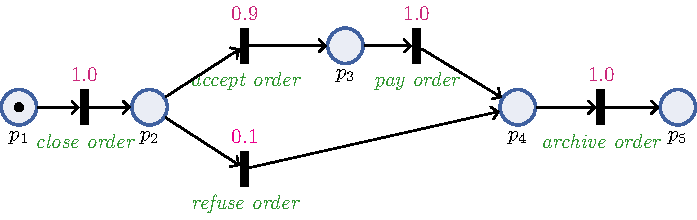
\includegraphics[width=.49\textwidth]{images/petri_tut.pdf}
	\caption{Stochastic Workflow Net modeling our use-case scenario.}\label{fig:petri_tut}
\end{figure}
\begin{figure}[!t]
	\centering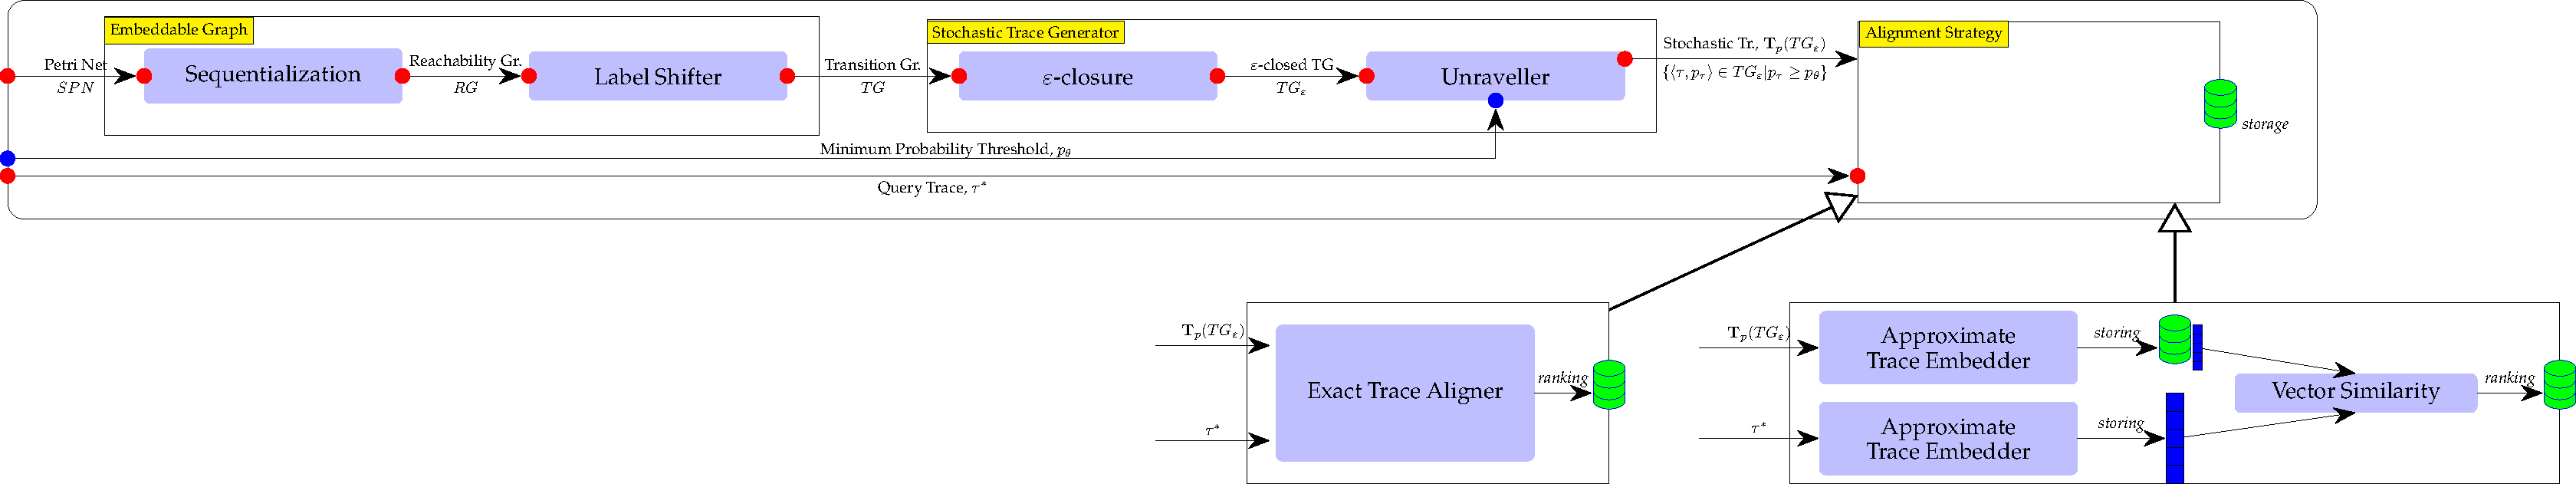
\includegraphics[width=.7\textwidth]{images/pipeline}
	\caption{Proposed pipeline to assess the probabilistic trace alignment.}\label{fig:pipe}
	\vspace*{-0.5cm}
\end{figure}

\section{Probabilistic Trace Alignment Pipeline}
%We now describe the proposed technique for computing probabilistic trace alignments. 
Our approach (\figurename~\ref{fig:pipe}) takes as input
\begin{inparaenum}[\it (i)]
	\item a reference model represented as an Stochastic Workflow Nets $\net$ or an equivalent Transition Graph $G$,
	\item a minimum, positive probability threshold $\pmin \in (0,1]$
	\item a trace $\trace$ of interest,
\end{inparaenum}
and returns a ranking over all the $\net$-traces having a probability greater than or equal to $\pmin$, based on a combined consideration of their probability values and their distance to $\trace$. First, we discuss input formats for \textit{(i)} as in the GUI.


%\section{Modeling Probabilistic Dynamic Systems}
%\label{sec:models}
%In this section, we introduce the different models and techniques that will constitute the basis for representing and computing probabilistic trace alignments.


%\subsection{Input}
%\subsection{Stochastic Workflow Nets}\label{subsec:spn}

\textbf{{Format: \texttt{Petri\_PNML}}.} Petri Nets and Generalized Stochastic Petri Nets are well-established formalisms \cite{DBLP:journals/tosem/PolyvyanyySWCM20} for modelling processes \cite{RoggeSoltiAW13} represented in the Petri Net Markup Language, supported by our tool. Due to the lack of space, we refer to \cite{spdwe} for the usual notation over Petri Nets. We restrict our interest to an interesting class of $1$-\textit{bounded} stochastic Petri nets with no timed transitions, namely \textsc{untimed Stochastic Workflow Nets} denoted as $N$. We now sketch the properties of the SWN accepted in PNML format and loaded as \textsf{PetriNet} objects: we consider two customary markings: the \emph{input} (resp.~\emph{output}) marking $m_{in}$ (resp.~$m_{out}$) assigning a single token to the input (resp.~output) place, and no token elsewhere. We assume to have a set $\alphabet = \tasks \cup \set{\tau}$ of labels, where labels in $\tasks$ indicate process tasks, whereas $\tau$ indicates an invisible execution step ($\tau$-transition). Labels are associated to transitions via a labelling function $\lambda$. A \emph{trace} is a finite sequence of labels from $\tasks$.
%\begin{definition} An \emph{untimed Stochastic Workflow Net (\uswn)}
%	is a tuple $\net = (P,T,F,\ell,W)$ where:
%	\begin{inparaenum}[\itshape (i)]
%		%\begin{inparaenum}
%		\item $(P,T,F)$ is a standard \emph{Workflow net} with places $P$, transitions $T$, and flow relation $F$ such that there is exactly one \emph{input place} with no incoming arc, and exactly one \emph{output place} with no outgoing arcs;
%		\item $\ell: T \rightarrow \alphabet$ is a \emph{labeling function} mapping each transition $t \in T$ into a label $\ell(t) \in \alphabet$ - this either indicates the task executed upon firing $t$, or the fact that $t$ is an invisible transition (in the latter case, $\ell(t) = \tau$);
%		\item $W\colon T\to \mathbb{R}^+$ is a \emph{weight function} assigning a positive firing weight to each transition of the net.
%	\end{inparaenum}
%\end{definition}
%Given an \uswn $\net$, we use dot notation to extract its constitutive components (e.g., $\net.P$ denotes its places). \emph{The same dot notation will be used for the other structures introduced in the paper}. We also use $\net.in$ and $\net.out$ to respectively denote the input and output place of $\net$.
The current state of execution is captured by a marking, i.e., a multiset of places $P$ indicating how many tokens populate each place.
%As pointed out above, \emph{we always assume, as customary in BPM, that the input \uswn is \underline{bounded}}, that is, in every state the number of tokens associated to each place cannot exceed a maximum, fixed threshold.
The notions of transition enablement and firing are also the standard ones  \cite{MarsanCB84}: %, which provides the basis for capturing the stochastic behavior of the net. 
%We use the following notation: given a marking $\marking$ over \uswn $\net$,  $\enaset{\marking}{\net}$ is the set of enabled transitions in $\marking$; given transition $t \in \enaset{\marking}{\net}$, we write $\fire{\marking}{t}{\marking'}{\net}$ to capture the fact that, with, firing $t$ in $\marking$ results in the new marking $\marking'$. A \emph{firing sequence starting from marking $\marking_0$} is a sequence $t_1\cdots t_n$ of transitions from $\net.T$ so that, for every $i \in \set{1,\ldots,n}$, we have that $\fire{\marking_{i-1}}{t_i}{\marking_{i}}{\net}$. We say that the firing sequence results in $\marking_{n}$.
%
given a marking $\marking$ %of $N$ 
and an enabled transition $t \in T_e$, the \emph{firing probability} of $t$ in $\marking$ is $\probt{t}{\marking}{\net} = \frac{W(t)}{\sum_{t'\in T_e}W(t')}$. %As required, 
The probabilities associated to all enabled transitions in a marking always add up to 1.
 A \emph{valid sequence} $\seq = t_1\cdots t_n$ is a firing sequence starting from $m_{in}^\net$ and resulting in $m_{out}$. The probability $\prob{\seq}{\net}$ of a valid sequence is the product of the probabilities associated to each transition: $\prob{\seq}{\net} = \prod_{i \in \set{1,\ldots,n}}\prob{t_i}{\marking_{i-1},\net}$. % A sequence of labels $\run = \alpha_1 \cdots \alpha_n$ from $\alphabet$ is a \emph{run} if there exists a valid underlying sequence $\seq = t_1\cdots t_n$  having $\alpha_i$ as a label for each $t_i\in \seq$. Run $\run$ may have different underlying valid sequences in $\seqs{\run}{\net}$.
  A trace $\trace=\const{a}_1\cdots \const{a}_m$ is a \emph{model trace} (or $\net$-trace for short) if there exists a valid sequence $\seq = t_1\cdots t_n$ where the appended labels $\lambda(t_1)\cdots \lambda(t_n)$ is equivalent to $\trace$ once all the $\tau$-s are stripped.
  %underlying run $\run$ corresponding to $\trace$ once all $\tau$ are removed. 
  There may be multiple valide sequences $\seq\in\seqs{\trace}{\net}$ %$\runs{\trace}{\net}$ 
  underlying an $\net$-trace $\trace$. 
   $\traces{\net}$ is the (possibly infinite) set of $\net$-traces. For a trace $\trace$ of $\net$, its probability $\prob{\trace}{\net}$ is then obtained by collecting all its underlying runs, in turn collecting all their underlying valid sequences, and summing up their respective probabilities: $\prob{\trace}{\net} = %\sum_{\run \in \runs{\trace}{\net}} 
   \sum_{\seq \in \seqs{\trace}{\net}} \prob{\seq}{\net}$. This corresponds to the intuition that, to observe $\trace$, one can equivalently pick any of its underlying valid sequences. Notably, if a trace is not an $\net$-trace (i.e., it does not conform with $\net$), then its probability is 0.
 These structural properties makes them suitable for loading BPMN nets as well: when the \texttt{Petri\_BPMN} is choosen, either the firing weight estimator is constant by default (\texttt{W\_CONSTANT}), or we can choose one from \cite{spdwe}. 
\begin{example} %\small
\label{ex:net}
\figurename~\ref{fig:spn} shows an example of an \uswn with input place $p_1$ and output place $p_7$. One run of the net is $\const{\tau c \tau a a \tau}$, which corresponds to trace $\const{caa}$. Overall, the net supports infinitely many finite traces of the form (represented using regular expressions):
\begin{inparaenum}[\it (i)]
\item $\const{aa^*}$,
\item $\const{cb}$,
\item $\const{caa^*}$.
\end{inparaenum}
\end{example}
%When executing an \uswn, the crucial addition to the standard execution semantics of Workflow nets is that, being the net stochastic, in each marking the set of enabled transitions gets associated to a discrete probability distribution. This is defined as follows: 
%given a marking $\marking$ of $N$ and an enabled transition $t \in \enaset{\marking}{\net}$, the \emph{firing probability} of $t$ in $\marking$ is $\probt{t}{\marking}{\net} = \frac{\net.W(t)}{\sum_{t'\in \enaset{\marking}{\net}}\net.W(t')}$. As required, the probabilities associated to all enabled transitions in a marking always add up to 1.
% %For a run $\run$ of $\net$, its probability $\prob{\seq}{\net}$ is then obtained by summing up the probabilities of all valid sequences corresponding to $\run$: $\prob{\run}{\net} = \sum_{\seq \in \seqs{\run}{\net}} \prob{\seq}{\net}$. Likewise, for a trace $\trace$ of $\net$, its probability is obtained by summing up
% For convenience, when needed, we represent an $\net$-trace as a pair $\tup{\trace,\prob{\trace}{\net}}$, where the probability assigned to $\trace$ by $\net$ is retained.


\textbf{Format: \texttt{StochasticMatrix}.} %\label{subsec:ppn}
The graph and trace embedding techniques %that we will use as the basis for computing probabilistic alignments 
cannot be directly defined over reachability graphs, as they %. In fact, these techniques 
rely on probabilistic \textsc{Transition Graphs} \cite{GartnerFW03} (class \textsf{ReadGraph}). Such graphs have transition probabilities associated to the edges, while nodes have labels in $\Sigma$, 
and represented via transition matrices. Each node is mapped by a matrix $L$ to a single label, as the same label may be used for multiple nodes, while a matrix $R$ represents a probability distribution over the next nodes to be picked upon executing a transition.
%where edges are only labeled by probabilities, whereas labels are attached to nodes. In addition, towards readily enabling efficient algorithmic techniques, such graphs are compactly defined using transition matrixes. We therefore take inspiration from \cite{GartnerFW03} and introduce the so-called \emph{probabilistic transition graphs}, which we will later use to encode \uswn{s} via their reachability graphs.
Due to the lack of space, we refer to \cite{GartnerFW03} for the standard notation for {probabilistic Transition Graphs}:
%For a matrix $Q$ with row set $A$ and column set $B$, notation $[Q]_{ab}$ for $a \in A$ and $b \in B$ denotes the corresponding element in the matrix. In addition $\transp{Q}$ denotes the transposed matrix where rows and columns are inverted. We employ the usual sum and product operations over matrixes and arrays, and denote, for a square matrix $Q$, the repeated multiplication of $Q$ with itself $n$ times by $Q^n$.\todo{Rimuovere questo paragrafo se serve spazio,}\todo{NOn si capisce il significato di $\omega$}
%In our technical treatment, we continue to assume the existence of a set $\alphabet$ of labels (including the special label $\tau$).
%\begin{definition} A \emph{(Probabilistic) Transition Graph} is a tuple $(V,s,t,L,R)$ where:
%	\begin{inparaenum}[\itshape (i)]
%		\item $V \subset \mathbb{N}$ is a set of \emph{nodes};
%		\item $s\in V$ is the \emph{initial node};
%		\item $e\in V$ is the \emph{accepting node};
%		\item $L: \alphabet \times V \rightarrow \{0,1\}$ is a \emph{label matrix} associating each node in $V$ to a single label in $\alphabet$, where for label $\alpha \in \alphabet$ and node $\ind{i} \in V$, $[L]_{\alpha\ind{i}}$ gives $1$ if $\ind{i}$ is labeled by $\alpha$, $0$ otherwise;
%		\item $R: V \times V \rightarrow [0,1]$ is a \emph{(probabilistic) transition matrix} indicating, for each pair of nodes, what is the probability that executing a transition from the first node leads to the second node.
%		% \item $\omega \in [0,1]$ is a \emph{graph weight} indicating an overall value associated to the entire graph.
%	\end{inparaenum}
%	$L$ and $R$ satisfy the following well-formedness conditions:
%	\begin{inparaenum}[\itshape (i)]
%		\item for every $i \in V$ there is one and only one label $\alpha \in \alphabet$ so   that $[L]_{\alpha\ind{i}}=1$;
%		\item  for  every $\ind{i} \in V$, we have that $\sum_{\ind{j}\in V}[R]_{\ind{ij}}=1$.
%	\end{inparaenum}
%\end{definition}
%The condition for $L$ indicates that 
matrices $L$ and $R$ can be exploited to determine the probability of reaching a node labeled by $\beta\in\Sigma$ from any node labeled $\alpha\in\Sigma$ in $n$ steps with $[LR^n\transp{L}]_{\alpha\beta}/[L\transp{L}]_{\alpha\alpha}$, that we can shorthand as $[G.\Lambda^n]_{\alpha\beta}$ \cite{GartnerFW03}.
%
A transition graph $\tg$ can be visualized as shown in \figurename~\ref{fig:lmc}. Still, %The various elements have the obvious interpretation %, with the only important consideration 
%that 
an edge from node $\ind{i}$ to node $\ind{j}$ is only shown if the transition probability $[\tg.R]_{\ind{i}\ind{j}}$ is positive.
%There, each node $\ind{i} \in \tg.V$ is  represented as a circle with its identifying number. The initial node is decorated by a small incoming edge, while the final node is double circled. The label of the node is shown close to the circle, in agreement with $\tg.L$. Finally, an edge from $\ind{i} \in \tg.V$ to $\ind{j} \in \tg.V$ is shown if the transition probability $[\tg.R]_{\ind{i}\ind{j}}$ is positive. Each edge is decorated with the positive probability assigned by $\tg.R$.
%\begin{definition}[Path, trace]
%A \emph{path} in a transition graph $\tg$ is a finite sequence of nodes $\ind{i}_1 \cdots \ind{i}_n$ (with $n > 1$) such that, for every $j \in \set{1,\ldots,n-1}$, we have that $[\tg.R]_{\ind{i}_j\ind{i}_{j+1}} > 0$. Such a path is \emph{valid} if it starts from the initial node and ends in the accepting node of $\tg$, that is, $\ind{i}_1 = \tg.s$ and $\ind{i}_n = \tg.e$.
%
%A \emph{trace} is a finite sequence of nodes that can be turned into a valid sequence by introducing in the sequence an arbitrary number of $\tau$ labels (so as to account for hidden transitions in the graph).
%\end{definition}
%From the definition, it is clear that every valid path can be straightforwardly converted into a corresponding trace by removing all $\tau$ labels from the sequence.
%$\npath{\ind{i}}{\ind{j}}$
%By mirroring to definitions of \uswn{s} taking into account that now labels are on nodes, a \emph{valid sequence} of $\tg$ is a sequence $\ind{i}_0\ldots\ind{i}_n$ of nodes in $\tg.V$ that leads from the initial to the accepting node by only traversing transitions with nonzero probability. 
%\begin{inparaenum}[\it (i)]
%	\item $\ind{i}_0 = \tg.s$;
%	\item $\ind{i}_n = \tg.e$;
%	\item if the sequence contains at least two nodes, each two consecutive nodes are connected by a positive transition probability, i.e., for every $j \in \set{1,\ldots,n}$ we have $[R]_{\ind{i}_{j-1}\ind{i}_{j}} > 0$.
%\end{inparaenum}
Valid sequences and model traces as well as their probability are defined similarly from \uswn{s}, and we employ the same notation. Matrices as well as Linear Algebra operations are implemented using sparse matrices and vectors from Eigen3.

%We close this section by introducing how some  matrix operations defined in the literature \cite{GartnerFW03} are applied to matrixes $L$ and $R$ of $\tg$, towards tackling interesting probability computations. These will be instrumental later on in the paper. Given two nodes $\ind{i},\ind{j} \in \tg.V$, $[R^n]_{\ind{i}\ind{j}}$ returns the probability of having a path in $\tg$ that connects $\ind{i}$ to $\ind{j}$ and has length $n$. Given two labels $\alpha,\beta \in \alphabet$, with $[LR^n\transp{L}]_{\alpha\beta}/[L\transp{L}]_{\alpha\alpha}$, we obtain the probability that, starting in any node labeled by $\alpha$, we reach a node labeled by $\beta$ through  $n$ consecutive steps in $\tg$. As a shortcut notation, we call the result $[\tg.\Lambda^n]_{\alpha\beta}$. Since there may be different nodes labeled by $\alpha$, we need to normalize the resulting probabilities. This is obtained with the division by $L\transp{L}$, which does so by assuming a uniform distribution when picking from which specific $\alpha$-labeled node one wants to start. Notice that these calculations need to be refined so as to consider proper runs and  traces. This will be done in Section~\ref{subsec:as}. %\todo{Rimandare alla sezione giusta}



%
%$\texttt{\color{blue}i}\overset{n}{\rightsquigarrow}\texttt{\color{blue}j}$ of length $n$: therefore, $[\Lambda^n]_{\color{green}\alpha\beta}:=[LR^nL^t]_{\color{green}\alpha\beta}/[LL^t]_{\color{green}\alpha\alpha}$ denotes the probability that, having started at any node labeled $\color{green}\alpha$ and taking $n$ steps, we arrive at any node labeled $\color{green}\beta$ (${\color{green}\alpha}\overset{n}{\rightsquigarrow}{\color{green}\beta}$). We denote as ${\color{green}\alpha}{\rightsquigarrow}{\color{green}\beta}$ an aforementioned path of arbitrary length.
%We can also associate a weight $\omega\in[0,1]\subseteq\mathbb{R}$ to a TG, so to express the probability associated with the TG itself as valid.
%




%\begin{example}
%We can graphically represent such TG as in \cite{Myers1989}.
%Figure \ref{fig:orig} is a  TG $P^*=(\mathtt{\color{blue}1},\mathtt{\color{blue}8},L,R,1)$ where $\omega=1$, where the matrices $L$ and $R$ can be both defined as follows:
%$$L:=\kbordermatrix{
%             & \texttt{\color{blue}1}&\texttt{\color{blue}2}&\texttt{\color{blue}3}&\texttt{\color{blue}4}&\texttt{\color{blue}5}&\texttt{\color{blue}6}&\texttt{\color{blue}7}&\texttt{\color{blue}8}&\texttt{\color{blue}9}&\texttt{\color{blue}10}\\
%\color{green}\varepsilon  & \textbf{1}&0&0&0&0&0&\textbf{1}&\textbf{1}&\textbf{1}&\textbf{1}\\
%\color{green}a            & 0&\textbf{1}&0&\textbf{1}&0&\textbf{1}&0&0&0&0\\
%\color{green}b            & 0&0&0&0&\textbf{1}&0&0&0&0&0\\
%\color{green}c            & 0&0&\textbf{1}&0&0&0&0&0&0&0\\
%}\qquad R:=\kbordermatrix{
%& \texttt{\color{blue}1}&\texttt{\color{blue}2}&\texttt{\color{blue}3}&\texttt{\color{blue}4}&\texttt{\color{blue}5}&\texttt{\color{blue}6}&\texttt{\color{blue}7}&\texttt{\color{blue}8}&\texttt{\color{blue}9}&\texttt{\color{blue}10}\\
%\texttt{\color{blue}1}  & 0&0&{\color{red}p_2}&0&0&0&0&0&{\color{red}p_1}&0\\
%\texttt{\color{blue}2}  & 0&0&0&0&0&{\color{red}p_3}&{\color{red}p_6}&0&0&0\\
%\texttt{\color{blue}3}  & 0&0&0&0&0&0&0&0&0&{\color{red}1}\\
%\texttt{\color{blue}4}  & 0&0&0&0&0&{\color{red}p_3}&{\color{red}p_6}&0&0&0\\
%\texttt{\color{blue}5}  & 0&0&0&0&0&0&0&{\color{red}1}&0&0\\
%\texttt{\color{blue}6}  & 0&0&0&0&0&{\color{red}p_3}&{\color{red}p_6}&0&0&0\\
%\texttt{\color{blue}5}  & 0&0&0&0&0&0&0&{\color{red}1}&0&0\\
%\texttt{\color{blue}8}  & 0&0&0&0&0&0&0&0&0&0\\
%\texttt{\color{blue}9}  & 0&{\color{red}1}&0&0&0&0&0&0&0&0\\
%\texttt{\color{blue}10}  & 0&0&0&{\color{red}p_4}&{\color{red}p_5}&0&0&0&0&0\\
%}$$
%\end{example}

% Given a TG $P=(s,t,L,R,\omega)$, a trace $\tau$ is a tuple in $(\Sigma\backslash\{\varepsilon\})^*$ denoting a path always originating from $s$ and terminating in $t$.
%\subsection{Input Transformation}
\medskip

\textbf{Transforming SWN$\to$TG.} If input is provided as a SWN $N$,  we internally represent all transition firings of an \uswn, together with their probabilities, in a reachability graph $RG(N)$ (\figurename~\ref{fig:rg} and \texttt{PetriMatrix} file format) by interpreting concurrency by interleaving. The transition probability function $P$ assigns to each transition an edge probability in $RG(N)$ as customary.  Due to the lack of space, we skip the customary definition of $RG(N)$.
%\begin{definition}
%The \emph{Reachability Graph} $\rg{\net}$ of \uswn \net is a triple $(M,E,P)$ where:
%\begin{compactitem}[$\bullet$]
%\item $M$ is the set of all reachable markings from $\marking_0^\net$ (including $\marking_0^\net$ itself).
%\item $E \subseteq M \times \alphabet \times M$ is a $\alphabet$-\emph{labeled transition relation} induced by $\net$, that is, for $\marking,\marking' \in M$, we have edge $(\marking,a,\marking') \in E$ if and only if there exists transition $t$  with label $\ell(t) = a$ and such that $\fire{\marking}{t}{\marking'}{\net}$.
%\item $P:E \rightarrow [0,1]$ is the \emph{transition probability} function assigning to each transition $(\marking,a,\marking') \in E$ its corresponding probability, obtained from the firing probability of the \uswn transition(s) that lead from $\marking$ to $\marking'$ and are labeled by $a$: $P(\marking,a,\marking') = \sum_{t_i \in \enaset{\marking}{\net} \text{ s.t.~} \net.\ell(t) = a \text{ and } \fire{\marking}{t}{\marking'}{\net}} \prob{t}{\marking}{\net}$.
%\end{compactitem}
%\end{definition}
%We now need to consider that, 
For a given state, distinct net transitions with the same label might produce the same consequent state, thus becoming indistinguishable from the trace perspective as they collaps into a single edge of the reachability graph. So, we accumulate all their firing probabilities into a single edge value. 
%Next, we handle %need to cope
%%Notice that, in the definition, 
%%we have to account for the possible case where, in a given state, 
%equivalently-labeled distinct net transitions from a given state % with the same label 
%producing the same consequent state: %. In this case, 
%as they are indistinguishable at the trace level by % when observing the execution traces of the net, and in fact they 
%collapsing into a single edge of the reachability graph, %. This is why, in this case, 
%we accumulate all their firing probabilities into a single value.
%
%In the remainder of the paper, 
Given an \uswn $\net$, we always assume that, in addition to its boundedness %, it the following structural assumptions that are natural in the BPM setting:
%\begin{compactitem}
%\item $\net$ is \emph{bounded}, that is, every marking in $\rg{\net}$ assigns at most a pre-defined number of tokens to each place;
%\item 
$\rg{\net}$ does not contain loops where all edges are labeled with $\tau$.
%\end{compactitem}
%The first assumption indicates that a case of the process does not generate unboundedly many parallel threads, and guarantees in turn that the reachability graph contains finitely many states. The second assumption naturally corresponds to how $\tau$-transitions are used when modeling business processes, where they are essential in representing gateways (such as exclusive and parallel splits/joins), cascaded gateways without tasks in between, and skippable tasks.  In all these cases, 
Multiple $\tau$-transitions may be used, but never creating completely invisible loops. {The absence of loops that solely go through $\tau$-transitions is reasonable modeling wise (as skipping multiple times an entire loop iteration is conceptually not distinguishable from not skipping it at all - so we would require there the presence of at least a visible activity witnessing that the iteration was executed, possibly skipping parts of it)}. Under this assumption, % $\net$ enjoys a very interesting property:
 there are only boundedly many valid sequences that can produce a given  trace $\trace$. The probability of $\trace$ can be computed by:
\begin{inparaenum}[\it (i)]
\item exhaustively enumerating all its valid sequences;
\item calculating the probability of each such sequence;
\item summing up all the so-obtained probabilities.
\end{inparaenum}
We directly encode \textsf{PetriNet}s to \textsf{ReadGraph}.
%\figurename~\ref{fig:rg} shows an example of a reachability graph.
\begin{example} %\small
  \label{ex:trace}
Consider the \uswn \net of Example~\ref{ex:net}. Considering trace $\const{caa}$, it is easy to see that it has only one underlying run, namely $\const{\tau c \tau a a \tau}$, in turn produced by a single underlying valid sequence, and that
%The firing probability of picking the first $\tau$-transition starting from the input marking is $1$, as there are no alternatives. In the new marking, where only one token is assigned to $p_2$, the firing probability of choosing the $\tau$-transition above is $\rho_{23} = \frac{v_{\tau_2}}{v_{\tau_2}+v_c}$, whereas that of choosing the $c$-transition below is $\rho_{24} = \frac{v_c}{v_{\tau_2}+v_c}$. Upon choosing the transition below, the new marking assigns only to $p_4$ one token, leaving just one choice to continue by moving that token to $p_6$. In that marking, the probability of choosing the $a$-transition above is $\rho_{65} = \frac{v_{a_3}}{v_{a_3}+v_b}$, resulting in the token being moved to $p_5$. In this new marking, the probability of iterating over the $a$-transition above is $\rho_{55} = \frac{v_{\tau_3}}{v_{\tau_3}+v_{a_2}}$, while that of completing in the output marking via the enabled $\tau$-transition is $\rho_{57} = \frac{v_{\tau_3}}{v_{\tau_3}+v_{a_2}}$. Hence, all in all
$\prob{\const{caa}}{\net} = 1 \cdot \rho_{24} \cdot 1 \cdot \rho_{65} \cdot \rho_{55} \cdot \rho_{57}$.
\end{example}



%Technically:
%\begin{compactitem}
%\item $P$ is a finite set of \textit{places}.
%\item $T$ is a finite set of \textit{transitions}, each of which is associate to a label. Each label either denotes a task executed upon transition firing, or indicates an invisible transition; in the latter case, we employ the special label $\varepsilon$.\footnotesize{This corresponds to the standard notion of $\tau$-transitions in Petri nets, but we use $\varepsilon$ since in the remainder of the paper $\tau$ is used to refer to an execution trace.}
%%to which we associate a label $\lambda(t)\in\Sigma$, where $\Sigma$ also includes the empty string\footnote{Given that we are going to denote the traces as $\tau$ and $t$ as the Petri net Transitions, we choose to denote the empty string as such instead of $\tau$ as in current literature from Petri nets.} $\varepsilon$.
%\item $F\subseteq (P\times T)\cup (T\times P)$ is the flow relation, representing arcs linking places to transitions and transitions to places.
%%to which we associate a \textit{firing cost} $\omega\colon F\to\mathbb{N}$.
%\item The initial place $i\in P$ has no ingoing edges ($\not\exists t\in T. (t,i)\in F$).
%\item The final place $f\in P$ has no outgoing edges ($\not\exists t\in T. (f,t)\in F$).
%\item $W\colon T\to \mathbb{R}^+_{>0}$ defines a \textit{firing weight} associated to each transition.
%\end{compactitem}

%A \textit{marking} is an assignment of a given amount of indistinguishable tokens to places described by a vector $M\colon P\to \mathbb{N}$. We say that a given transition $t$ is \textit{enabled} if $M(p)\geq 1$ for each ingoing $p$ to $t$ ($(p,t)\in F$). If such transition is enabled, then it can \textit{fire} a token. The \textit{enabling transitions} $E(M)$ for a given marking $M$ are all the $t$ reachable from $p$ ($(p,t)\in F$) with $M(p)\neq 0$ where $t$ is enabled. When $t$ can fire a token for a marking $M$, we can generate a novel marking $M'$ from $M$ by moving the tokens from the ingoing places towards the outgoing places as follows:
%\[\forall p\in P.\; M'(p)=M(p)-\mathbf{1}_{(p,t)\in F}+\mathbf{1}_{(t,p)\in F}\]
%We denote the transition from marking $M$ to marking $M'$ via an enabling $t$ as a relation $M\overset{t}{\to}M'$. We say that an \uswn with initial marking $M$ is $k$-\textit{bounded} if each of the markings $M'$ reachable from $M$, $M$ included, have $\forall p\in P.\; M(p)\leq k$\\

\begin{figure*}[!t]
	\begin{minipage}{.49\textwidth}
		\centering
		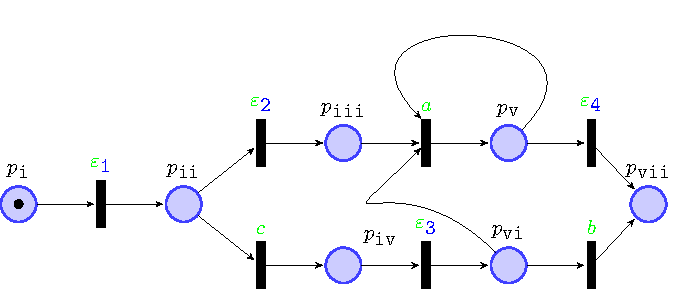
\includegraphics[width=.7\textwidth]{images/petri.pdf}
		\caption{A sample \uswn. Labels are shown in green, $\tau$ transitions in grey, weights in magenta.}\label{fig:spn}
	\end{minipage}\hfill \begin{minipage}{.49\textwidth}\centering
		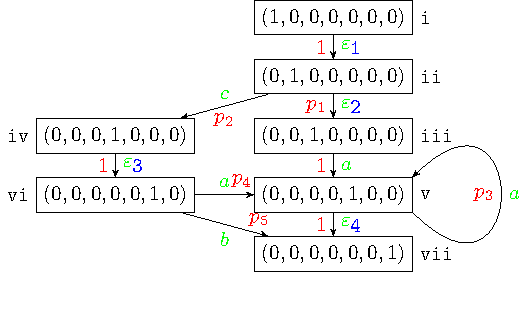
\includegraphics[width=.8\textwidth]{images/rg.pdf}
		\caption{Reachability graph $RG(N)$ of the \uswn $N$. Probabilities are shown in violet.}\label{fig:rg}
	\end{minipage}
\end{figure*} \begin{figure*}[!t]
	\begin{minipage}{.49\textwidth}\centering 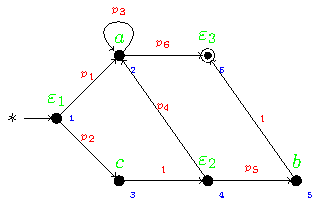
\includegraphics[width=.55\textwidth]{images/running_example.pdf}
	\caption{Transition graph $G_{RG(N)}$ encoding the reachability graph $RG(N)$.}\label{fig:lmc}\label{fig:orig}
\end{minipage}\hfill \begin{minipage}{.49\textwidth}\centering 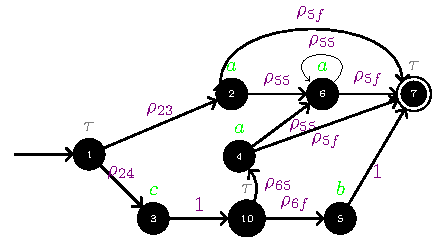
\includegraphics[width=.55\textwidth]{images/closed_example.pdf}
	\caption{Transition graph $\closed{G_{RG(N)}}$ resulting from the transition graph in $G_{RG(N)}$ after $\tau$-closure.}\label{fig:closed}
\end{minipage}
\end{figure*}


%Figures \ref{fig:spn} and \ref{fig:rg} respectively show a sample \uswn and its corresponding reachability graph. This net will be our running example throughout the paper.


%\begin{example}
%Figure \ref{fig:spn} provides a sample \uswn defined as such, and \ref{fig:rg} provides its associated Reachability Graph. This representation can be beneficial when such \uswns are inferred and extracted from log files \cite{PPNFromLog} for extracting the set of the probabilistic traces associated to the \uswn.
%\end{example}
%
%
%We use \uswns for modelling business processes: in fact, it can be shown \cite{RaedtsPUWGS07} that it is always possible to convert BPMNs to \uswns. Last, we also assume that a transition is enabled when all of its input places contain at least one token and that, when a transition fires, we remove one token from each of its input places and depose tokens for each of its output places.

We can show that there exists a conversion from $\rg{\net}$ (\figurename~\ref{fig:rg}) into a transition graph $\tg_{\rg{\net}}$ (\figurename~\ref{fig:orig}) preserving model traces as well as their probabilities via well-known techniques used to \emph{shift labels} from automata theory.  


\textbf{$\tau$-closure} The resulting transition graph $\tg_{\rg{\net}}$ is processed applying a \emph{$\hidden$-closure} that compiles away
$\tau$-transitions. This results into a new transition graph $\closed{\tg_{\rg{\net}}}$ (\figurename~\ref{fig:closed}) %that on the one hand only retains
retaining $\hidden$ labels only in the initial and accepting states while, for the rest, it exclusively operates over visible labels in $\tasks$. %, and, on the other, continues to preserve model traces and their probabilities. Also in this case we omit the details, as 
The transformation relies on well-known automata-based techniques for removing $\epsilon$-moves while preserving model traces, as well as their associated probabilities. %The only non-trivial observation is that, even in our case where probabilities are present, 
All $\tau$ transitions can still be removed thanks to the working hypothesis done for \uswn{s}, as no loops can contain only $\tau$ transitions. %The transition graph in \figurename~\ref{fig:orig} results in that of \figurename~\ref{fig:closed}.
\medskip

\textbf{Unfolding.} Next, we efficiently unfold the previously closed graph to collect TG-traces having probability greater or equal than $\pmin$ (\textsf{Minimum trace probability}) via the Eigen3 linear algebra library. Unfolding is efficiently performed via sparse matrices for TGs over the Eigen library. %The $\hidden$-closed transition graph $\closed{\tg_{\rg{\net}}}$ is \unravelled, so as to collect all the model traces that have a probability of at least $\pmin$. To do so, we rely on a key property that $\closed{\tg_{\rg{\net}}}$ inherits from the fact that it results from an \uswn. 
Since an \uswn has a Workflow net as underlying control-flow structure and given that TG inherits the results from SWNs, no loop can be executed without strictly decreasing the resulting probability. So, all valid sequences with a resulting probability of at least $\pmin$ can be enumerated and returned in a set. The so-obtained sequences are then combined by merging those that produce the same trace, summing up their probabilities, thus obtaining the set of all the traces having a probability greater than or equal to $\pmin$, $\ptraces{\closed{\tg_{\rg{\net}}}}{\pmin}$. The closure operation also implies that the notion of model trace collapses with the one of run modulo removing the initial and the final $\tau$ labels attached to the initial and accepting nodes. %In addition to that, traces might be also pre-filtered by \textsf{Maximum complete trace length}. 
\medskip
